\section{Objetivos}
 O objetivo principal desta prática é a implementação da convolução como ferramenta matemática para obtenção da saída de um sistema dada uma entrada qualquer e a resposta ao impulso.
 
\section{Fundamentação Teórica}
A convolução, pode-se assim dizer, é o equivalente entre sinais da multiplicação. Ela pode ser descrita em tempo contínuo, sendo chamada de integral de convolução e em tempo discreto de soma de convolução.

\subsection{Integral de convolução}
A resposta $y(t)$ a uma entrada $x(t)$ aplicada a um sistema T, sendo este linear e invariante no tempo, pode ser dado pela Equação \ref{Convolucao_continuo}, onde $h(t)$ é a resposta do sistema ao impulso. Esta dedução partiu da propriedade da função impulso dada na Equação \ref{definicao_delta}.

\begin{equation}
	x(t) = \int_{-\infty}^{\infty}x(\tau)\delta(t-\tau)d\tau
    \label{definicao_delta}
\end{equation}

\begin{eqnarray}
    y(t) &=& T{x(t)} \nonumber\\
    y(t) &=& T{\int_{-\infty}^{\infty} x(\tau)\delta {t-\tau}d\tau} \nonumber\\
    y(t) &=& \int_{-\infty}^{\infty} x(\tau)T{\delta {t-\tau}}d\tau \nonumber\\
    y(t) &=& \int_{-\infty}^{\infty} x(\tau)h{t-\tau}d\tau \nonumber\\
    y(t) &=& x(t)*h(t)
    \label{Convolucao_continuo}
\end{eqnarray}

\subsection{Soma de convolução}
A resposta em tempo discreto, $y[n]$, a uma entrada $x[t]$ aplicada a um sistema T, sendo este linear e invariante no tempo, pode ser dado pela Equação \ref{Convolucao_discreto}, onde $h[n]$ é a resposta do sistema ao impulso. Esta dedução partiu da propriedade da função impulso dada na Equação \ref{definicao_delta_discreto}.

\begin{equation}
	x[n] = \sum_{-\infty}^{\infty}x[k]\delta(n-k)
    \label{definicao_delta_discreto}
\end{equation}

\begin{eqnarray}
	y[n] &=& T{x[n]} \nonumber\\
	y[n] &=& T{\sum_{-\infty}^{\infty} x[k]\delta [n-]} \nonumber\\
    y[n] &=& \sum_{-\infty}^{\infty} x[k]T{\delta [n-k]} \nonumber\\
    y[n] &=& \sum_{-\infty}^{\infty} x[k]h[n-k] \nonumber\\
    y[n] &=& x[n]*h[n]
    \label{Convolucao_discreto}
\end{eqnarray}

\section{Procedimentos}
Foram resolvidos os exercícios 1 2 da apresentação de slides referente a transformada Z, com código implementado em Matlab.

\subsection{Exercício 1}
Determine a saída do sistema com
resposta ao impulso h[n] e para um sinal de entrada
x[n], ambos sinais estão mostrados na Figura \ref{fig:procedimento_pr1_ex1}:\\
A) análise gráfica por impulsos \\
B) cálculo/tabela de convolução \\
C) convolução utilizando ferramenta
computacional: \emph{script} Matlab

\begin{figure}[!th]
	\centering
    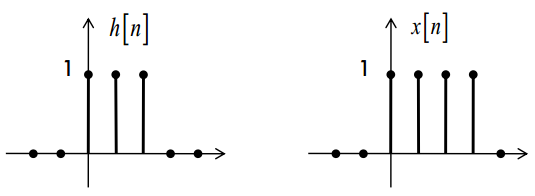
\includegraphics[scale = .7]{Imagens/Execicio1.PNG}
    \caption{Sinais do Exercício 1, prática 1.}
 \label{fig:procedimento_pr1_ex1}
\end{figure}

\subsection{Exercício 2}
Considere um sistema que possui resposta
ao impulso h[n]=$2^{-nT}$ e o sinal de entrada é uma onda
retangular (razão cíclica 40\%, D=0,4) com período
10s e amplitude 3,3V.\\
A) Determine a resposta (sinal de saída) do sistema para
3 períodos do sinal de entrada considerando que o
periodo de amostragem é T=0.2s.\\
B) Considere um ruído de 10\% no sinal de entrada e
repita o item A.\\
C) Considere um sinal de entrada senoidal com mesmo
período, amplitude e ruído dados acima.

\section{Resultados e discussões}

\subsection{Exercício 1}
\subsubsection{C)}
O código implementado em Matlab para a resolução da letra C do exercício 1 está logo abaixo:
\lstinputlisting{Arquivos_tex/Aula_3_Exercicio_1.m}

Obtendo como saída o gráfico da Figura \ref{saida_ex1_pr_1}

\begin{figure}
	\centering
    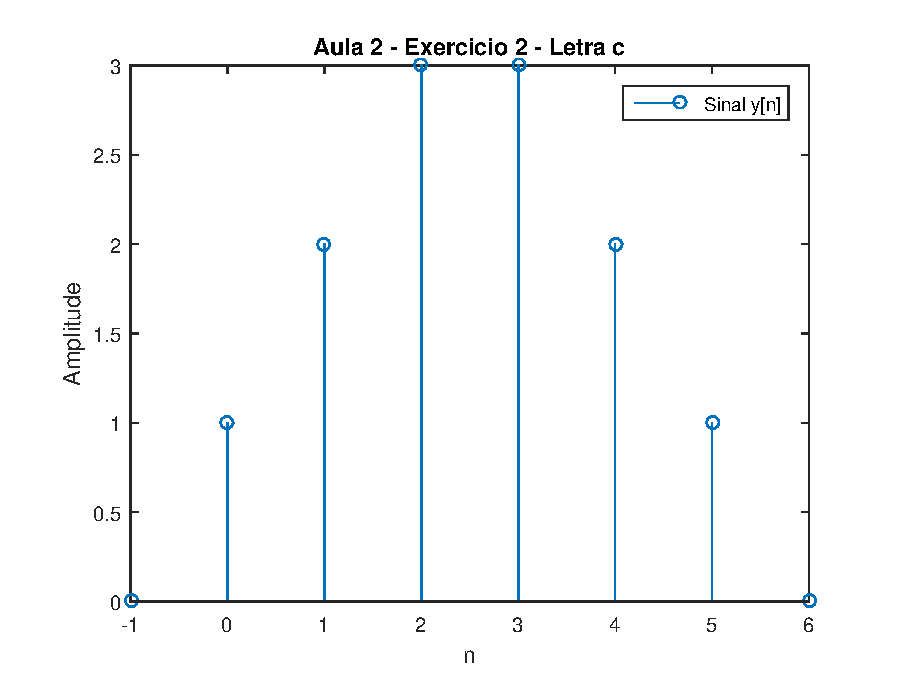
\includegraphics[scale = .7]{Imagens/Aula_3_exercicio1_LetraC.eps}
    \caption{Gráfico de saída do código do Exercício 1, letra C, prática 1.}
    \label{saida_ex1_pr_1}
\end{figure}

Observa-se que os intervalos de simulação para uma convolução teórica deveria ser estabelecido entre $- \infty$ e $+ \infty$, com uma valor de passo unitário. Porém computacionalmente esses intervalos são impraticáveis, necessitando de uma adequação nos valores de simulação.

Como os sinais $h$ e $x$  possuem valores diferentes de zero apenas a partir de $n~=~0$ até $n~=~3$ se faz necessário convolucionar apenas neste intervalo. O numero total de pontos convolucionados é dado pela soma dos valores no intervalo da convolução dos dois sinais, sendo portanto no total 8 pontos.  

A figura \ref{saida_ex1_pr_1} apresenta o resultado da simulação de forma coerente com a teoria, e portanto comprova a eficacia do algoritmo desenvolvido. 

\subsection{Exercício 2}
O código implementado em Matlab para a resolução do exercício 2 está logo abaixo:
\lstinputlisting{Arquivos_tex/Aula_3_Exercicio_2.m}

Obtendo como saída os gráfico das Figuras \ref{saida_ex2_pr_1_L_A}, \ref{saida_ex2_pr_1_L_B} e \ref{saida_ex2_pr_1_L_C}. 

\begin{figure}[!ht]
	\centering
    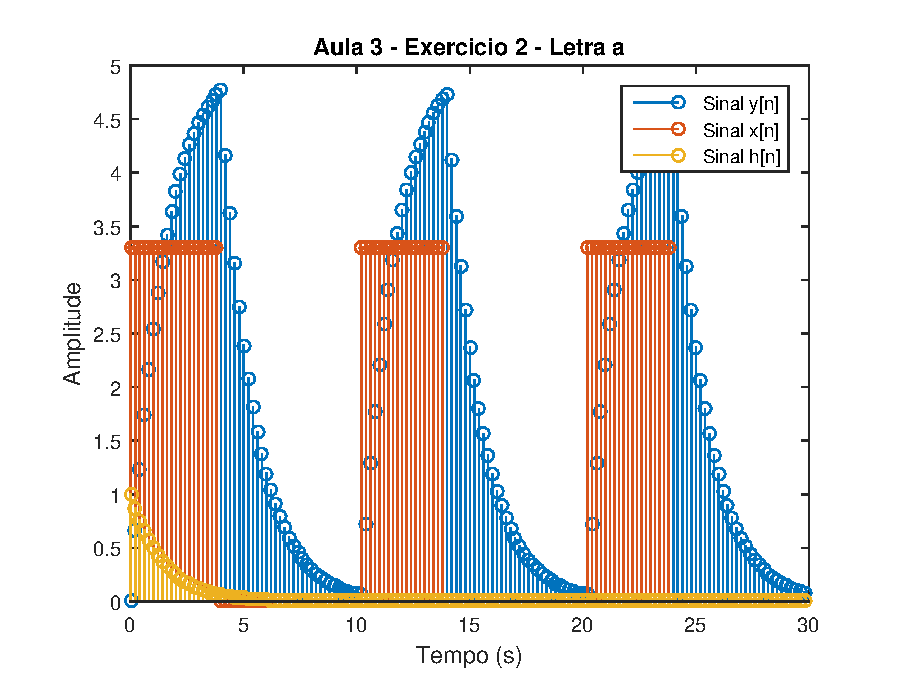
\includegraphics[scale = 1]{Imagens/Aula_3_exercicio2_LetraA.eps}
    \caption{Gráfico de saída do código do Exercício 2, letra A, prática 1.}
    \label{saida_ex2_pr_1_L_A}
\end{figure}

\begin{figure}[!ht]
	\centering
    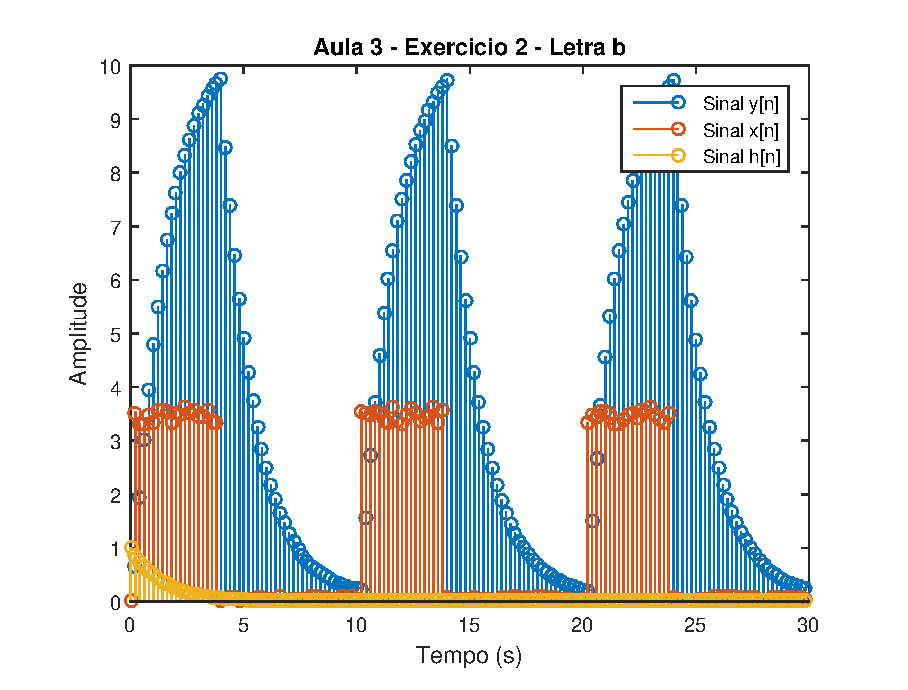
\includegraphics[scale = 1]{Imagens/Aula_3_exercicio2_LetraB.eps}
    \caption{Gráfico de saída do código do Exercício 2, letra B, prática 1.}
    \label{saida_ex2_pr_1_L_B}
\end{figure}

\begin{figure}[!ht]
	\centering
    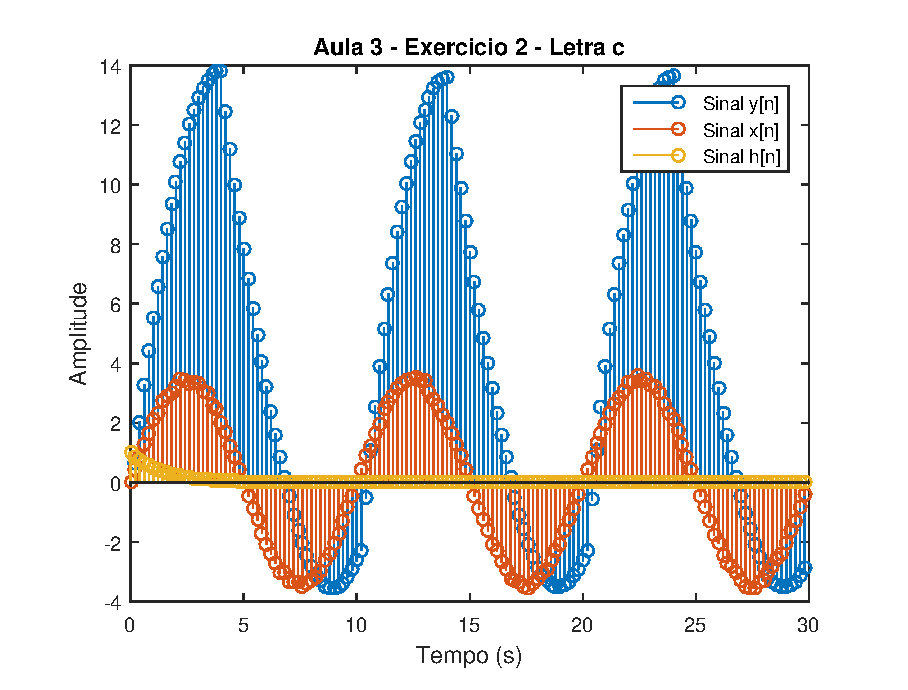
\includegraphics[scale = 1]{Imagens/Aula_3_exercicio2_LetraC.eps}
    \caption{Gráfico de saída do código do Exercício 2, letra C, prática 1.}
    \label{saida_ex2_pr_1_L_C}
\end{figure}

Neste exercício deve se ter umas atenção especial em relação ao passo da convolução, ou seja a quantidade de pontos simulados entre valores inteiros.  

Como temos um período de amostragem de $0,2$ logo temos 5 pontos simulados  entre valores inteiros. Assim se fixarmos o numero de períodos e variarmos o número de amostragem variamos também o número  de pontos a serem convolucionados. Como a convolução pode ser representada pela soma na forma da equação \ref{Convolucao_discreto}, logo a amplitude de cada ponto $n$ do sinal convolucionado depende do numero de amostras realizado. Para que se possa ter um sinal de amplitude normalizada independente do período de amostragem,  o sinal convolucionado é dividido pelo numero de amostras entre intervalo entre dois inteiros, ou numero de amostras por ciclo.